\documentclass[12pt,twocolumn,a4paper]{article}
\usepackage{layout}
\usepackage[utf8]{inputenc}
\usepackage{url}
\usepackage{latexsym}
\usepackage{amsmath, amsthm, amsfonts}
\usepackage{graphicx}
\usepackage{geometry}
\usepackage{dirtytalk}
\usepackage{ragged2e}
\usepackage[colorlinks = true,
           linkcolor = black,
           urlcolor  = black,
           citecolor = blue,
           anchorcolor = blue]{hyperref}
\geometry{
	paper=a4paper, 
	top=3cm, 
	bottom=4cm, 
	left=2.0cm, 
	right=2.5cm, 
	headheight=0.75cm,
	footskip=1.5cm,
	headsep=0.75cm, 
}
\usepackage{setspace}
\setstretch{1.0}
\usepackage{enumitem}
\setlist{noitemsep}

\renewcommand{\thesection}{\Roman{section}}
\renewcommand{\thesubsection}{\arabic{subsection}} 
\renewcommand{\thesubsubsection}{\alph{subsubsection}}

\begin{document}
    
    %cover page
    \begin{titlepage}
        \newgeometry{top=1.5cm, 
        	bottom=3cm, 
        	left=2.5cm, 
        	right=2.5cm}
        \onecolumn
        \begin{center}
            
\includegraphics[height=25mm]{ksu_masterlogo_colour_rgb.png}
            \vspace{0.3cm}
            
            \Large
            King Saud University \\
            College of Computer and Information Sciences\\
            Computer Science Department
            
            \vspace{2.5cm}
            \Huge
            \textbf{AI with Computer Vision: A Literature Review}
                
            \vspace{3.0cm}
            \Large
            \textbf{\textit{Prepared By:}\\ 
                Nouf Alsubaie \hspace{65pt}  441200911\\
                Fatimah Alhumaidhi \hspace{10pt}  441200921\\
                Layan Alarifi \hspace{75pt}  441201121\\}
            \vspace{2.5cm}
            \Large
            \textbf{\textit{Supervised By:}\\
                T. Nouf Alshenaifi}
            
            \vfill
            First Semester 1444/2022
        \end{center}
    \end{titlepage}
    
    \restoregeometry
    \twocolumn
    \justifying
    %sections
    \section{Introduction}
    \hspace{0.3cm} Artificial intelligence (AI) is a field of computer science that concentrates on making intelligent agents that are capable of thinking and reasoning rationally to solve different problems \cite{Russell2020-tt}. Artificial intelligence is inter-related with other subfields like machine learning and deep learning. Nowadays, AI became a wide area of research, it includes the study of many important topics like natural language processing (NLP), expert systems, speech recognition and computer vision. AI has many useful applications in real life and it provides effective solutions in business, transportation, health care, and other fields.
    
    In 1959, Arthur Samuel created the subject of study known as machine learning (ML), a subfield of computer science that enables computers to learn from experience without being explicitly programmed \cite{Samuel1959-rx}. This concept can also refer to the procedure of gathering data and algorithmically creating a statistical model based on that data in order to solve a real-world problem \cite{Burkov2019-rd}. Computers can now complete tasks like (classification, clustering, prediction, pattern recognition, etc.) thanks to the development of ML. ML algorithms can be categorized into four groups based on the learning method: supervised learning, unsupervised learning, semi-supervised learning, and reinforcement learning.
    
    In supervised learning, the machine learns how to map the input into output after observing a number of examples that explicitly show what is the correct output for each input \cite{Russell2020-tt}. In practice, this means that supervised learning needs labeled datasets in order to train the model. While in unsupervised learning the machine recognizes patterns in the input data and draws conclusions without explicit feedback given to the machine \cite{Russell2020-tt}. Thus, in an unsupervised approach, there is no need to provide labeled datasets. 
    
    Computer Vision is a field that is concerned with acquiring, analyzing, and processing digital images and videos via computers. Computer vision first emerged in the early 1970s and was thought of as the visual perception part of an ambitious plan to imitate human intelligence and give machines intelligent behavior. The desire to retrieve three-dimensional structure from images with the aim of obtaining a full scene understanding distinguished computer vision from the predominant field of digital image processing \cite{Szeliski2011}.

    Applications of computer vision in artificial intelligence (AI) and machine learning (ML) have received a great deal of attention in recent years as a result of recent advancements in computer hardware and parallel processing, some of computer vision applications in AI include: Object recognition, Image Generation and Image Classification. In this review, we talk about each of these applications in depth, showing how they are applied and used, and when were they invented. We also talk about the latest technologies used in the field and explain how they work.
    
    \section{Literature Review}
    \subsection{Object Recognition}
    \hspace{0.3cm} Recognition is a visual ability that includes identification and discrimination between different objects \cite{Liter1998-bk}. The term object recognition in computer vision refers to the task of identifying an object and categorizing it as an instance of a certain class \cite{Liter1998-bk}. The goal is to find a correspondence between some of the image features with similar features in the object model \cite{Mutihac2005PARADIGMSIO}. The main problem in object recognition is to determine which features to use and how to obtain the correspondence between the image and the model.

    Based on the available information about the object, there are two types of object recognition; model-based object recognition and view-based object recognition. In the first type, a 3D model is available representing detailed information about the object parts, shape and how different parts are combined. On the other hand, the view-based recognition lacks a fully described 3D model, instead, it maintains some information about how the object looks from different view angles and uses these data to recognize the object \cite{Mutihac2005PARADIGMSIO}.

    Before the rise of deep learning, scientists had to apply classical machine learning approaches to extract the image features manually before training the model \cite{Varadarajan2021-po}. This required researchers to have extensive domain knowledge in order to design a detection algorithm that looks for predefined features in an image, yet these models do not achieve the required accuracy and are still vulnerable to mistakes if the image size or resolution has changed \cite{Goyal2014-xk}. However, the use of deep learning models has led to great improvement in object recognition.

    The main advantage of deep learning models over traditional learning models is that in deep learning the algorithm can learn from the data itself without human supervision. This is done by using highly connected parallel networks known as neural networks which are inspired from the human nervous system and brain. The neural network consists of multiple layers. In each layer there are a number of nodes that perform a certain processing or computational operation, each node has dense interconnections with other nodes in the network \cite{Mutihac2005PARADIGMSIO}.

    Since the deep learning models are data-driven, we no longer need to extract features manually \cite{Mutihac2005PARADIGMSIO}. The model can automatically extract the features by processing the images and recognizing the pixel pattern that made up a certain object. In this way, the model can learn by itself which features to look for to recognize the object. There are many techniques and models in deep learning, but some of them have shown significant improvement when used in computer vision applications. Convolutional Neural Networks (CNNs) and Deep Belief Networks (DBNs) are widely used in the computer vision field \cite{Voulodimos2018-cu}.

    Convolutional neural networks(CNNs) consist of three types of neural layers: (i) convolutional layers, (ii) pooling layers, and (iii) fully connected layers, each type of layers is responsible for different operation \cite{Voulodimos2018-cu}; The convolutional layer is what makes CNNs different from typical neural networks, it uses special image filters called kernels to extract image features and generating the feature maps, after the first convolutional layer only low-level features like edges and corners are extracted, then the output is fed again into another convolutional layer to extract higher-level features. The final reasoning is done by the fully connected layers that follow several convolutional and pooling layers \cite{Voulodimos2018-cu}. The CNN model is known for its capability in feature learning, However, a major drawback of CNN is that it relies on the existence of a labeled data set.

    Many works on object recognition apply CNNs. In a study conducted by Matija Radovic et al. \cite{Radovic2017-la}, a convolutional neural network model is trained on a set of aerial images including real-time video feed from unmanned aerial vehicles (UAVs). Due to the high speed of the UAV environment, the proposed model uses 26 convolutional layers instead of 24-configuration to increase the accuracy and the speed of the detection. the results show that the CNN was able to recognize “airplane” objects in the data set with 97.5\% of accuracy  while only 16 instances were incorrectly categorized (Figure \ref{fig:aa}).
    
    \begin{figure}[htp]
        \centering
        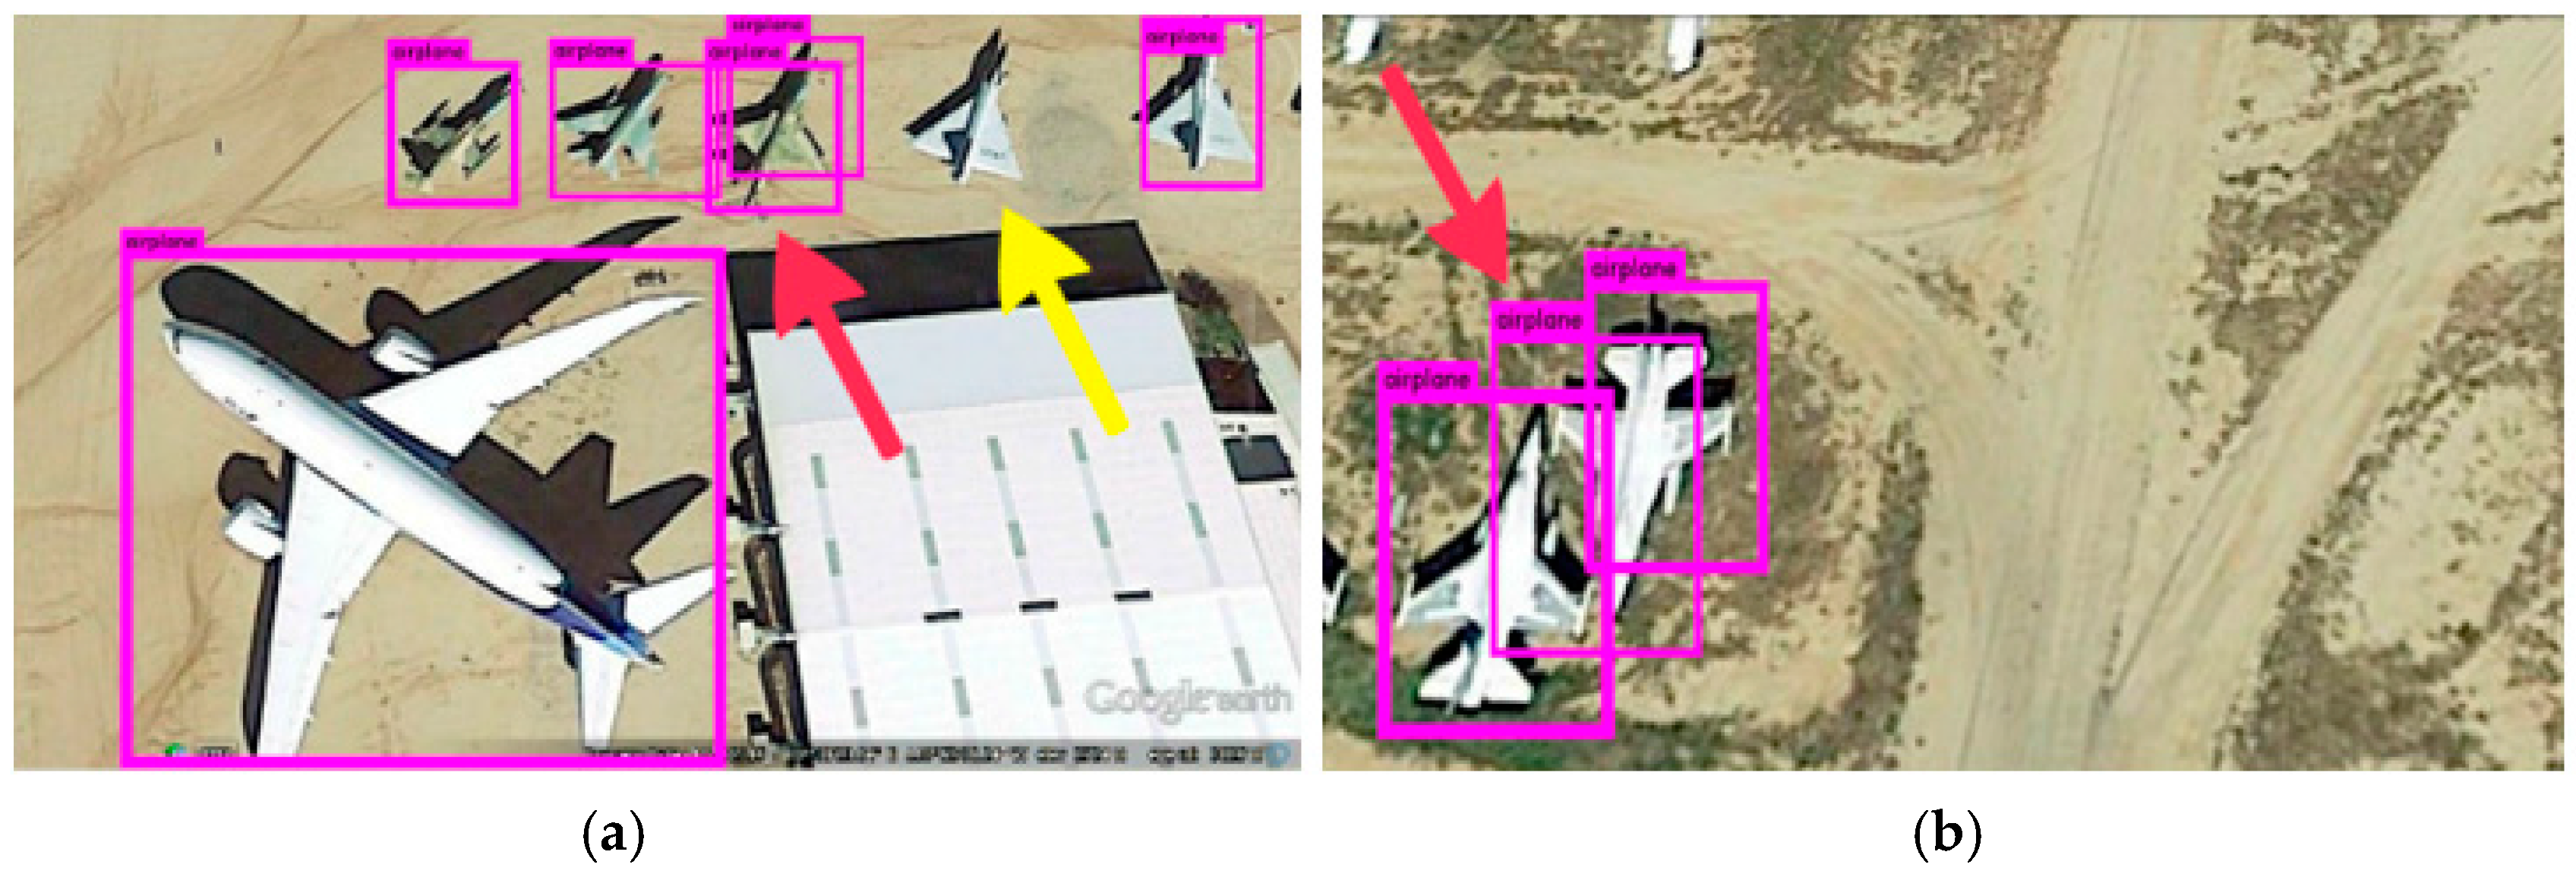
\includegraphics[scale=0.5]{jimaging-03-00021-g004.png}
        \caption{\centering . (a) Yellow arrow points at the instances where “airplane” object is present but not detected by the CNN, (b) red arrow points to the instance where “airplane” object is wrongly identified.\cite{Radovic2017-la}.}
        \label{fig:aa}
    \end{figure}

    Another research \cite{Bamba2021-kd} uses convolutional neural networks in the medical field to recognize anatomical objects in surgical real-time videos. The dataset videos used in the research were recorded during different surgeries carried out at a medical university in Tokyo. The model was trained to recognize different anatomical objects like blood, vessels, uterus, forceps, ports, gauze and clips in the surgical images. After training the model has achieved an accuracy of 83\% and precision of 80\%. which proves the efficiency of using CNNs in object detection. 

    Deep Belief Networks (DBNs) is a generative model structured by stacking multiple restricted Boltzmann machines (RBM) and training them in a greedy manner \cite{Voulodimos2018-cu}. The RBM is an undirected graphical model containing a set of stochastic visible variables and hidden variables such that each visible variable is connected to each hidden variable with a restriction that the connection between them must form a bipartite graph \cite{Voulodimos2018-cu}. The DBNs use RBM to initialize the deep network and then train the model using a greedy strategy. The main advantage of the above structure is that it solves the problem of selecting appropriate parameters and does not require labeled data since the process is unsupervised \cite{Voulodimos2018-cu}.

    As an example of using DBNs for object recognition; There is a study conducted to detect manipulation in satellite images using deep belief networks \cite{Horvath2020-qh}. The manipulation includes splicing images from different sources to generate manipulated images. The researchers train and test four different DBNs with the MINST data set. And found that the proposed model was able to detect and localize manipulation even with small forgeries \cite{Horvath2020-qh}.
    
    \subsection{Image Generation}
    \hspace{0.3cm} Image generation tasks are tasks where the goal is auto-generation of digital images or videos by a deep learning model. For this task, a network called Generative Adversarial Network (GAN) was first introduced in a 2014 paper by Goodfellow et al. \cite{Goodfellow2014-cu}. Generative Adversarial Networks are semi-supervised deep learning models that consist of two parts: a generative model and an adversary model, the generative model generates samples by passing random noise through a multilayer network, which then send the output to the adversary model. The adversary model is a discriminative model that learns to determine whether a sample is from the model distribution or the data distribution \cite{Goodfellow2014-cu}. this framework was based on the two-player minimax game with the following objective function:
     \begin{equation*}
        \begin{aligned}
        \min_{G}\max_{D} V(G,D) = \mathbb{E}_{x\sim pdata(x)}[\log D(x)] +\\
        \mathbb{E}_{z\sim pz(z)}[\log (1-D(G(z)))]
        \end{aligned}
     \end{equation*}
    where the discriminator D tries to maximize the probability of assigning the correct label to both training examples and samples from the generator, and the generator G tries to minimize the correct labels \cite{Goodfellow2014-cu}.\\
    \-\hspace{0.5cm} GANs showed great success in image generation tasks. Resent applications of image generation is concerned with generating images from text description, Zhang et al. \cite{Zhang2016-pu} used  a model called Stacked Generative Adversarial Network (StackGAN) to Synthesize lifelike images from English text description. Even with using deep learning models like GAN, generating images from text description is a hard task for a computer to process. In \cite{Zhang2016-pu}, the problem was divided into 2 smaller stages, where the first-stage GAN model creates the fundamental shape and colors of the object based on the provided written description, producing low-resolution pictures. The output of the first stage with the written description serve as inputs for the second stage of GAN, which creates high-resolution images with realistic looking qualities. With the refinement process, it is able to fix flaws in first-stage results and add interesting details to the image. Figure \ref{fig:bb} shows examples of some generated images by GAN models \\
        \begin{figure}[htp]
        \centering
        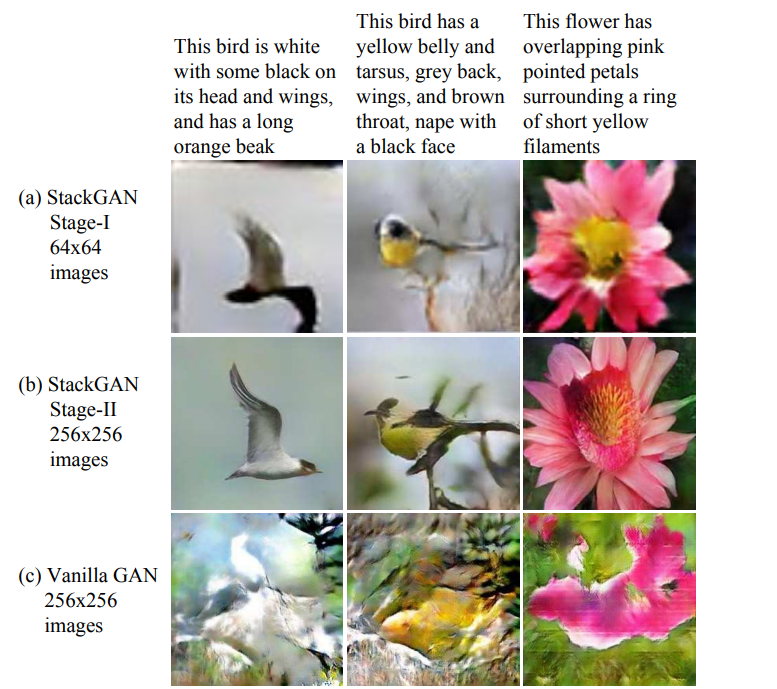
\includegraphics[scale=0.3]{birds.png}
        \caption{\centering Comparison of StackGAN and a vanillaone-stage GAN for generating images from text \cite{Zhang2016-pu}.}
        \label{fig:bb}
    \end{figure}
    
    deep generative models can be applied to many real-life tasks, a 2016 paper by Goodfellow \cite{Goodfellow2016} mentioned some of them:
    \begin{itemize}
    \item Super-resolution of a single image: The objective of this task is to create a high-resolution equivalent from a low-resolution image.
    \item Tasks where the goal is to create art.
    \item Applications of image-to-image translation can transform sketches into graphics or aerial photos into maps.
    \end{itemize}
    \-\hspace{0.1cm} Other important applications of generative models might include generating dataset for training other deep learning models. Deep generative models can be categorized according to how they can learn. Models that can learn using the concept of maximum likelihood have different representations or approximations of the likelihood. Figure \ref{fig:cc} shows a taxonomic tree of generative models that can learn using the concept of maximum likelihood.
    \begin{figure}[htp]
        \centering
        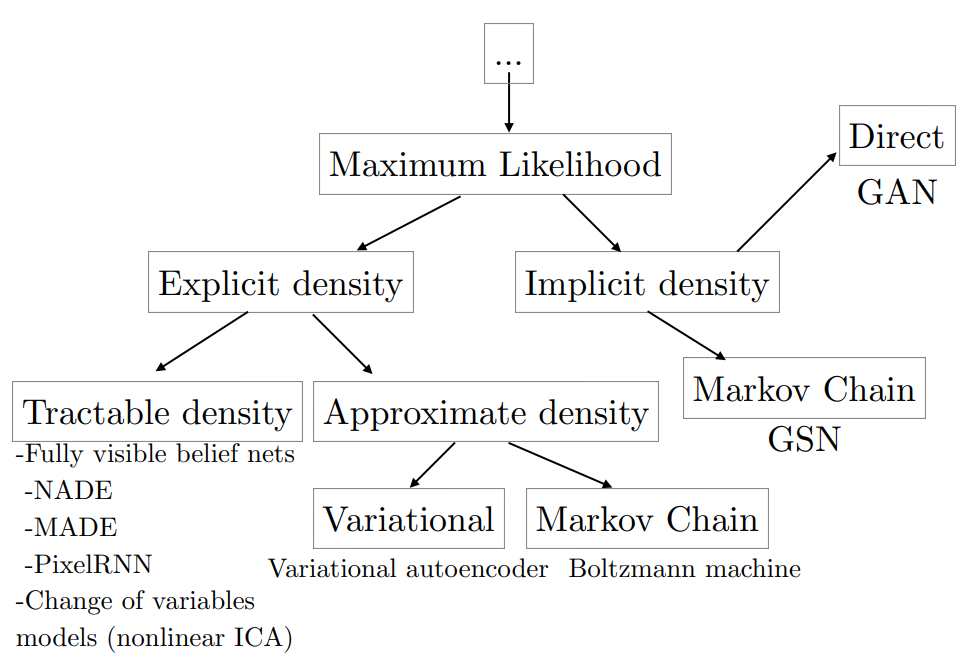
\includegraphics[scale=0.3]{generative-models.png}
        \caption{\centering Taxonomic tree of generative models \cite{Goodfellow2016}.}
        \label{fig:cc}
    \end{figure}
    
    \subsection{Image classification}
    \hspace{0.3cm} Image classification is a key task in computer vision that aims to annotate images with specific labels that describe their semantic information \cite{Wu2020-kx}. The semantic information is extracted from the underlying features of the image. This is done by training a classifier to learn from a data set and classify images using a specific classification algorithm \cite{Wu2020-kx}. 

    Image classification isolates the characteristic information in the image from color or shape and does not care, for example, about a flat background or noise.  AlexNet, VGG-16, GoogleNet, ResNet, Inception-V3 and DenseNet are all common neural networks models that can be used for image classification \cite{Gowda2019-rd}.

    Image classification can be divided into two problems: binary classification and multiclass classification.  Binary classification involves designating an input image into one of two classes, while in multiclass classification, two or more classes are included.  A classic example of a binary image classification problem is identifying cats or dogs in each input image.  Paper \cite{Gowda2019-rd} also mentioned that deeper networks and highly interconnected networks showed an evolution in the performance of image classification tasks, and with the progress, Image classification became of great importance for the developed dataset such as (SVHN, MNIST, CALTECH-101, CALTECH-256) It is noteworthy that most of the datasets are color where as stated in the paper \cite{Gowda2019-rd} \say{These color images are represented in RGB format.  Computer, these images are just numbers and have no inherent meaning in meaning. Most modern models developed for classification do not convert the color space to the image and instead use the RGB image directly for classification}. 
     
    \subsection{Face Recognition}
    \hspace{0.3cm} There are many technologies that help in identifying a person in recent years, for example, using fingers and hands for identification, but relying on this technique may not always be useful because it may be exposed to bruises or cracks, which hinders obtaining the desired results, and when using the eye through iris and retina techniques, it requires expensive equipment, and is very sensitive to any movement of the body, while the sound is also not always appropriate because it is subject to noise in public places, but the face images can be obtained easily using a pair of fixed cheap cameras. It doesn't take a lot of people to use the technology, unlike the above techniques \cite{10.3745/JIPS.2009.5.2.041}.

    Face recognition can be used for two tasks: 1- Verification, which is matching from one person to another, 2- Identification, and one-to-many matching, i.e. displaying an image of an unknown person and comparing it with a known database until that person is identified. They are applied and used for security, surveillance, public identity verification, image database investigations, and much more. Speaking of the difficulties with face recognition technology, differences in age, differences in lighting, and differences in pose are the main problems it suffers from \cite{10.3745/JIPS.2009.5.2.041}.

    Automatic face recognition in its early days was feature-based and used to measure distinctive facial features such as eyes, mouth, nose, etc., and then calculate geometric relationships between facial points, resulting in reduction of the input face image to a vector of geometric features, and then the face is recognized using standard statistical pattern recognition techniques \cite{10.3745/JIPS.2009.5.2.041}.

    Modern statistical methods and artificial intelligence methods attempt to identify faces based on the entire image rather than the local features of the face. Statistical methods obtain the results by direct correlation comparisons between the input face and all other faces in the dataset. On the other hand, AI methods use tools such as neural networks and machine learning techniques to recognize faces. The results were satisfactory and good as they were in equal lighting, size and appropriate setting, but it was computationally expensive, and its other drawback is that it is sensitive to changing light and noise and the direction of the face (Figure \ref{fig:dd}) \cite{10.3745/JIPS.2009.5.2.041}.

    \begin{figure}[htp]
        \centering
        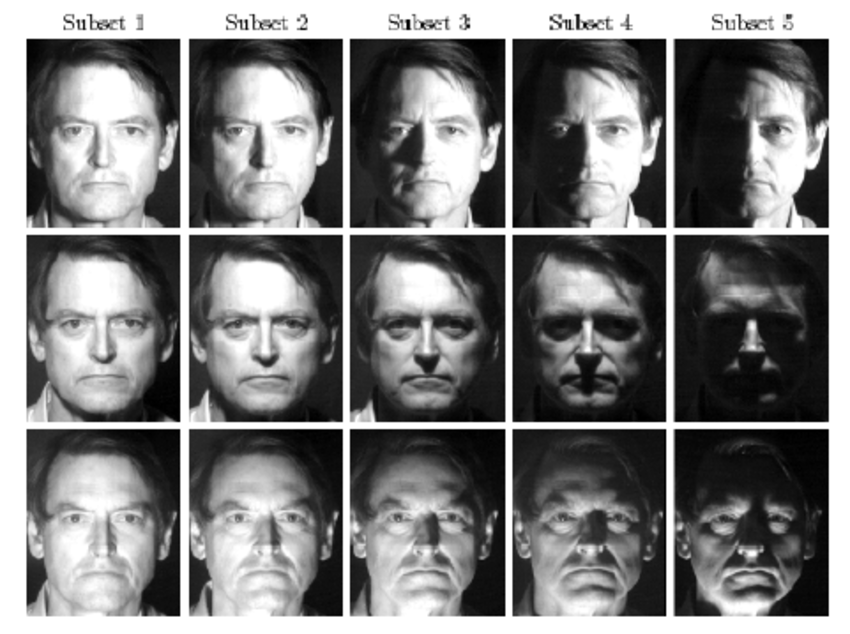
\includegraphics[scale=0.2]{face.png}
        \caption{\centering The same person seen under varying light 
conditions can appear dramatically different \cite{10.3745/JIPS.2009.5.2.041}.}
        \label{fig:dd}
    \end{figure}
    
    \section{Discussion}
    \hspace{0.3cm} Advances in artificial intelligence over the last few years have greatly improved the field of computer vision. As we reviewed the latest works in the computer vision field, we observed that deep learning models are widely used to perform different computer vision tasks like object recognition, image generation, and image classification. 

    In the past, scientists had to manually extract the image features before training their models using classical machine learning approaches, These models were susceptible to errors and highly affected by changes in the image size and resolution, So they failed to deliver the required accuracy. until the development of neural network models allows for more accurate performance. 
    
    In object recognition, many recent studies use convolutional neural networks (CNNs) and deep belief networks (DBNs) as the main methodology to recognize objects in real-life applications. CNNs are more commonly used when compared to DBNs. CNN approach is preferred for its unique capability in learning features and generating feature maps. However, the CNN model relies on the existence of a labeled data set in contrast to the DBN model which is unsupervised and can work with unlabeled data sets. 

    It is generally agreed that deep learning models can yield good results and achieve high accuracy, but the main limitation is the time complexity and the computational resources needed to train them. Since all data are interconnected the size and computation increase exponentially. Some researchers suggested removing connections between certain nodes and proposed other variations of the models to reduce the complexity \cite{Horvath2020-qh}.

    In addition, we note that most works on object recognition and image classification are usually an improvement on existing models. This improvement is in terms of increasing the accuracy or reducing the complexity of the model. While the image generation field is still inventing new models that perform hard tasks such as text-to-image generation. 


    \section{Conclusion}
    \hspace{0.3cm} The invention of deep neural networks has greatly improved our capability to perform computer vision tasks. Convolutional neural networks (CNNs) and deep belief networks (DBNs) are two NNs models that are widely used in the literature and have proven to be useful in many real-life applications. However, The exponential complexity and the high demand for computational resources are still unsolved limitations.
    
    Although computer vision is a well-established field with many successful studies, There are still some hard tasks that need to be studied and improved. Generative Adversarial Network (GAN) is a good example of a newly invented model that shows great success in image to text generation.
    
    %IEEE referencing Style
    \bibliographystyle{ieeetr}
    \bibliography{References}

\end{document}
